\section{Análisis Comparativo}
\begin{frame}
 \begin{center}
  \LARGE Análisis Comparativo
 \end{center}
\end{frame}
\begin{frame}
 \frametitle{Análisis Comparativo}
 \begin{itemize}[<+->]
  \item Existen muchos trabajos sobre distintas formas de comparar la seguridad de ambas plataformas.
  \item Esta tesina propone analizar distintas características presentes en ambas plataformas, \pause poniendo foco en \structure{los permisos que se pueden modificar \emph{en tiempo de ejecución}}.\pause
  \item Se analizaron cuatro características presentes en iOS y Andriod:\pause
     \begin{itemize}[<+->]
      \item Arranque verificado
      \item Cifrado del sistema de archivos
      \item Bloqueo del dispositivo
      \item Seguridad de las aplicaciones
     \end{itemize}
 \end{itemize}
\end{frame}
\begin{frame}
 \frametitle{Análisis Comparativo}
Se pone foco especialmente en los sistemas de permisos:\pause
 \begin{figure}[btp]
    \centering
    \begin{subfigure}{0.23\linewidth}
        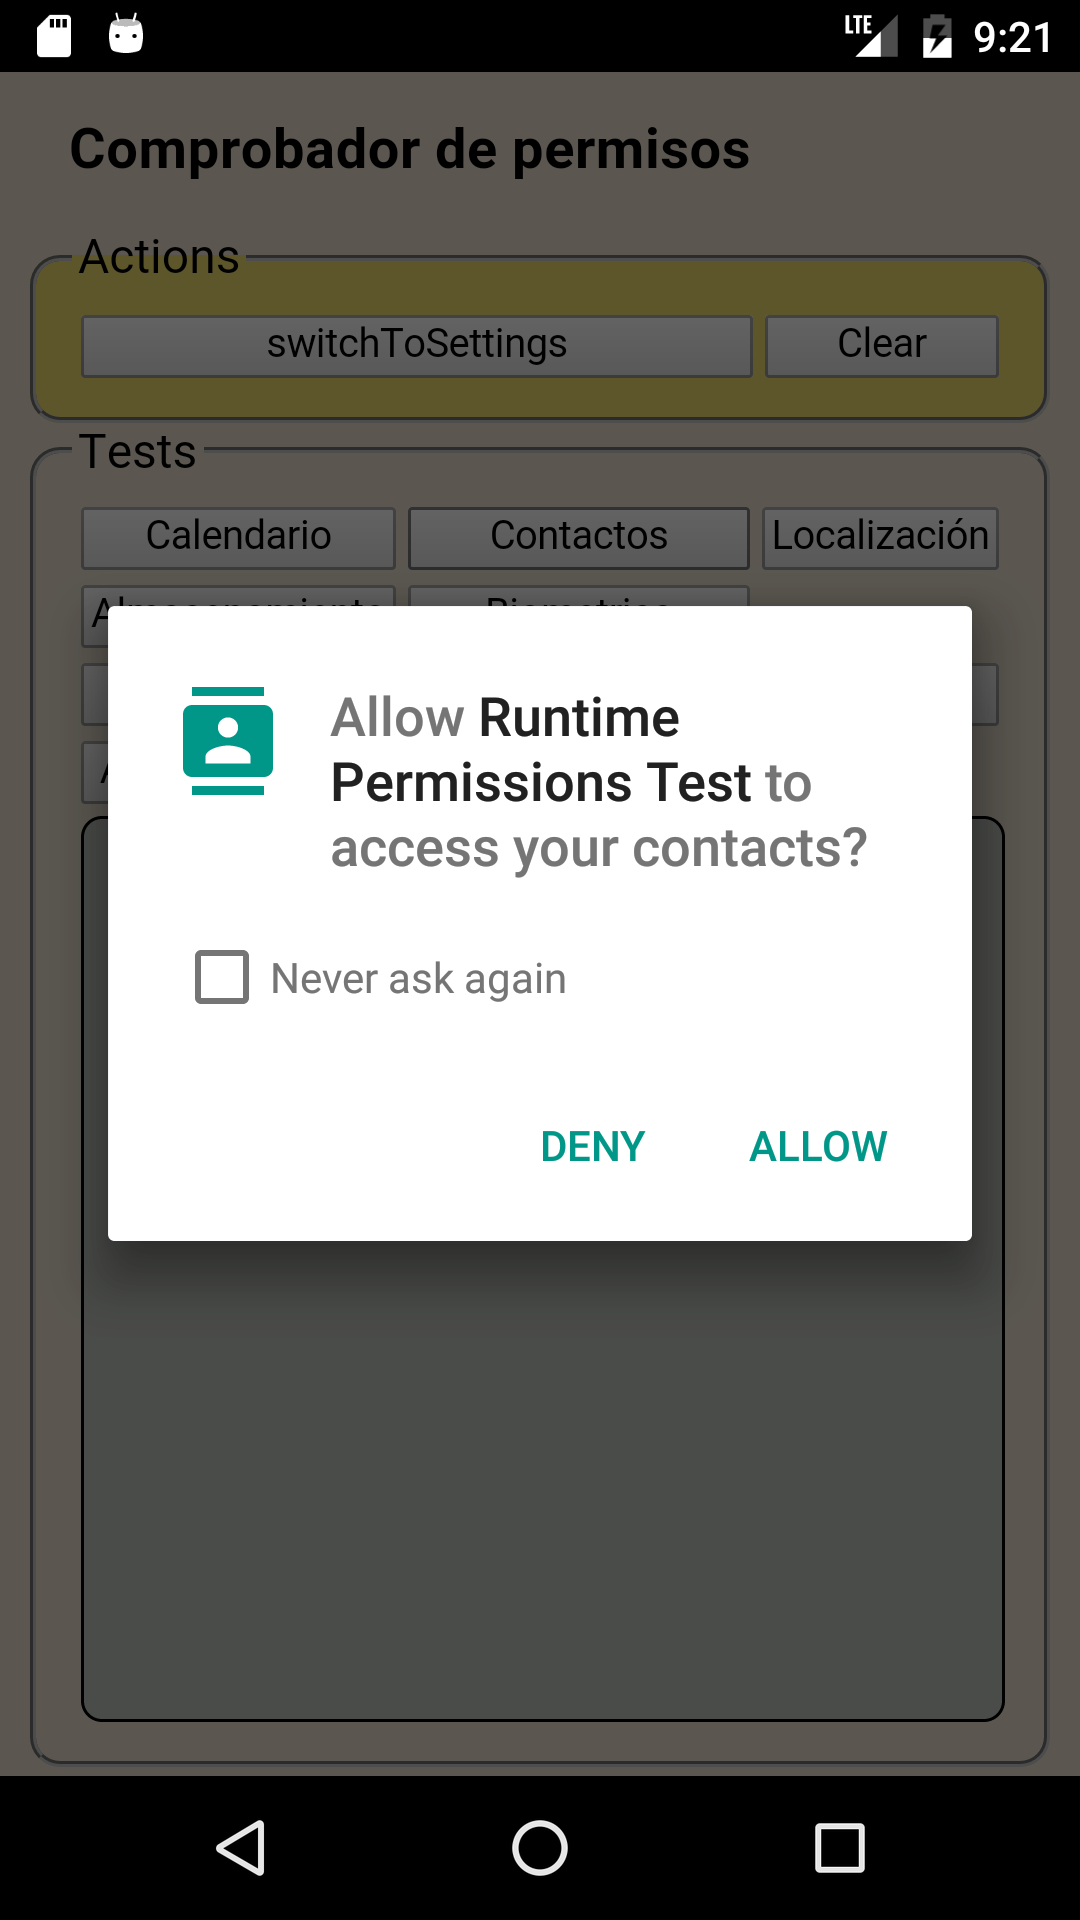
\includegraphics[width=\linewidth]{allow_contact}
        \caption{Pedido de un permiso en Android.}
    \end{subfigure}
    \begin{subfigure}{0.23\linewidth}
        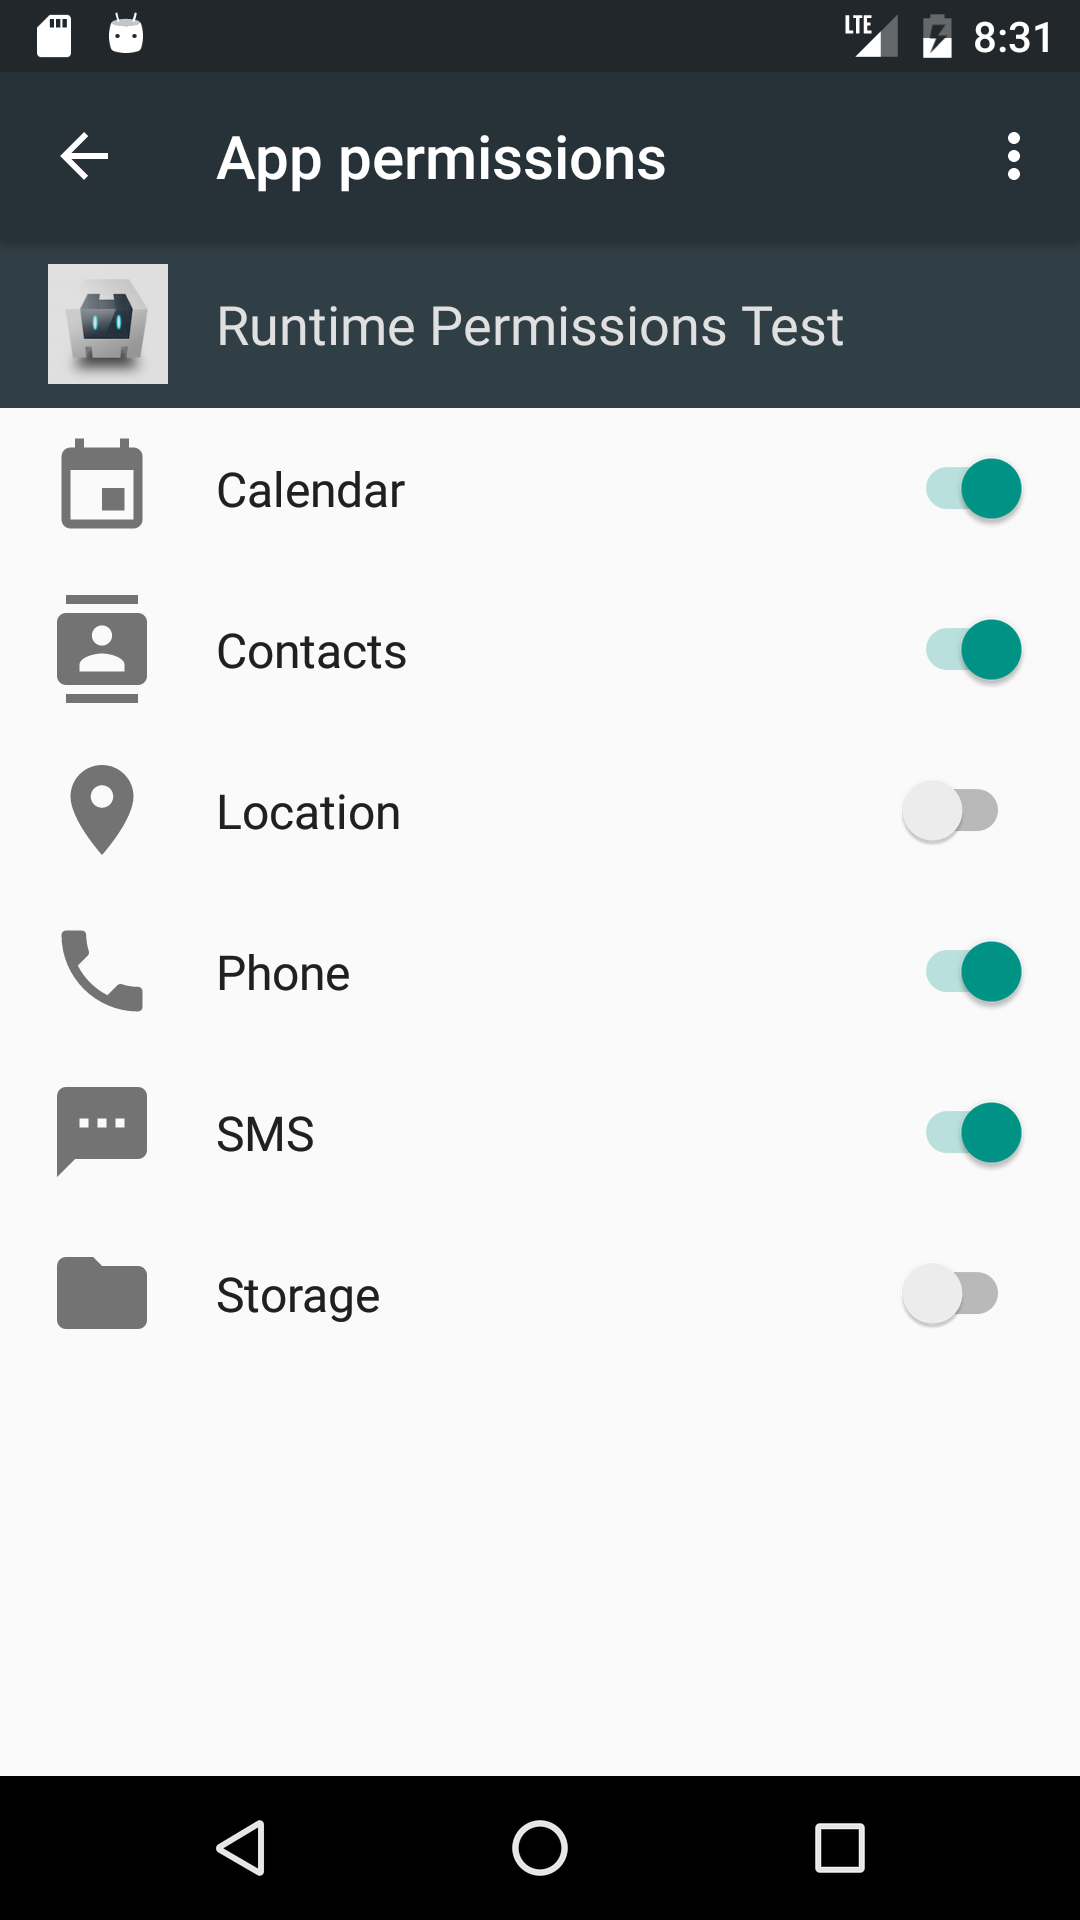
\includegraphics[width=\linewidth]{app-permissions}
        \caption{Sistema de permisos de Android.}
	\end{subfigure}\pause
	\begin{subfigure}{.23\linewidth}
    	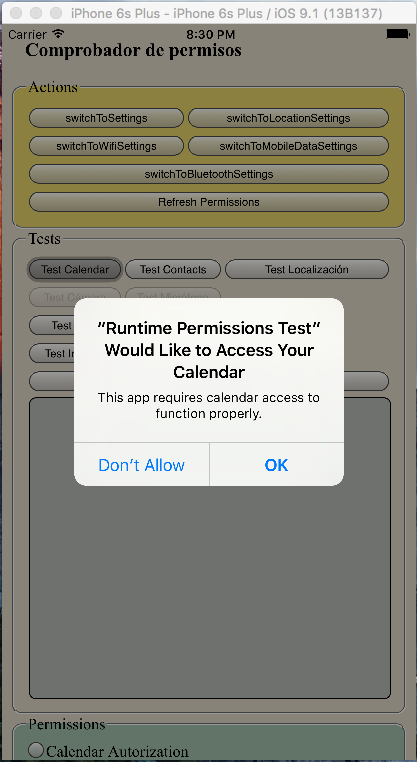
\includegraphics[width=\linewidth]{calendar_request_ios}
    	\caption{Pedido de un permiso en\\ iOS.}
    \end{subfigure}
    \begin{subfigure}{.23\linewidth}
    	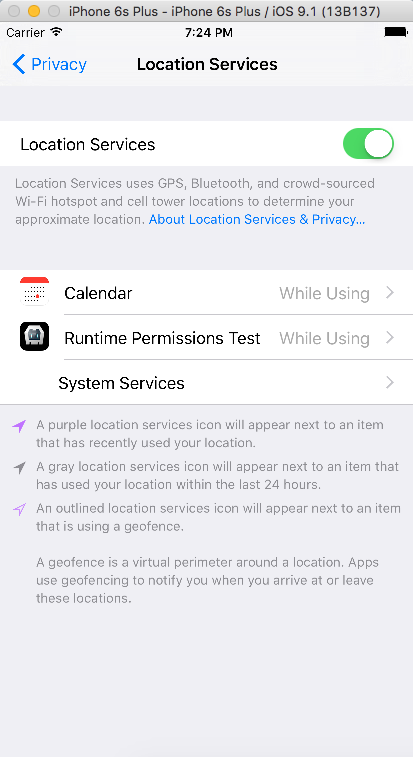
\includegraphics[width=\linewidth]{apps-allow-location}
    	\caption{Sistema de permisos de\\ iOS.}
	\end{subfigure}
	\caption{Permisos modificables en \emph{tiempo de ejecución}.}
\end{figure}
\end{frame}
\begin{frame}
 \frametitle{Análisis Comparativo}
Al comparar la gestión de permisos de ambas plataformas, encontramos varias similitudes:\pause
 \begin{itemize}[<+->]
  \item A una aplicación se le otorga permisos básicos al momento de instalación, sin posibilidad de revocarlos.
  \item Si una aplicación necesita un permiso no básico, debe requerirlo. El usuario puede otorgarlo o revocarlo.
 \end{itemize}
\end{frame}
\begin{frame}
 \frametitle{Análisis Comparativo}
Respecto a cómo se definen los permisos: \pause
 \begin{itemize}[<+->]
  \item En Android están orientados según el riesgo implícito al otorgarlos.
  \item En iOS los permisos están orientados a los componentes.
 \end{itemize} \pause
 \begin{tiny}
  \begin{table}[H]
    \centering
	\begin{tabular}{c c c}
		\hline
		\multicolumn{3}{c}{\textbf{Permisos}} \\
		\emph{Ambas plataformas} 	& \emph{Solo en Android}	& \emph{Solo en iOS} \\ \hline    \hline
		Calendario	& -		& -	\\						
		Contactos	& -				& - \\						
		Cámara		& -				& -	\\						
		Localización& -				& -	\\						
		-			& -				& Compartir por Bluetooth\\ 
		Micrófono   & -				& - \\						
		-			& Teléfono		& -	\\						
		Sensores    & -    			& - \\						
		-			& SMS			& - \\						
		-			& Almacenamiento& - \\						
		-			& -				& \emph{Homekit} \\			
		-			& -				& Redes Sociales \\        	
		-			& -				& Diagnóstico \\        			
		-			& -				& Publicidad \\    			\hline
	\end{tabular}
	\caption{Resultado de la comparación de permisos.}
   \end{table}
   	\end{tiny}
\end{frame}
\begin{frame}
 \frametitle{Análisis Comparativo}
Respecto del alcance del sistema de permisos:\pause
  \begin{itemize}[<+->]
   \item En Android, un permiso es a nivel de grupo. Por lo tanto, el usuario otorga o deniega para todo el grupo.
   \item La misma situación ocurre en iOS: se otorga un permiso de acceso a todas las funcionalidades de un determinado componente.
  \end{itemize}
\end{frame}
\begin{frame}
 \frametitle{Análisis Comparativo}
Si observamos la cobertura del sistema de permisos, \pause las dos plataformas dejan funcionalidades sin permisos modificables \emph{en tiempo de ejecución}:\pause
  \begin{itemize}[<+->]
   \item En Android se destacan: Acceso a Internet, Compartir vía Bluetooth e Información del Dispositivo.
   \item En iOS se destacan: Acceso a Internet y SMS. Tampoco tiene la suficiente granularidad para administrar el acceso a los datos de las llamadas telefónicas.
  \end{itemize}
\end{frame}
\begin{frame}
 \frametitle{Análisis Comparativo}
\small {Para finalizar se analizará la interacción con el usuario:}\pause
\begin{figure}
	\centering
	\begin{subfigure}{.23\linewidth}
		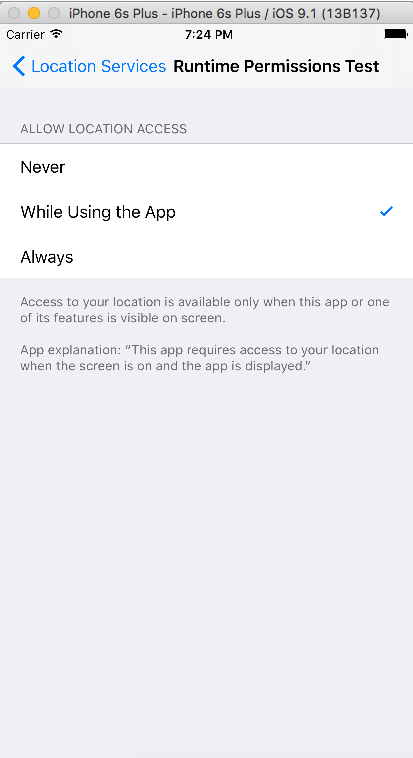
\includegraphics[width=\linewidth]{permission-classes.png}
		\caption{Permisos requeridos por una aplicación.}
		\label{fig:ch05:ios_all_permissions}
	\end{subfigure}\pause
	\begin{subfigure}{.23\linewidth}
		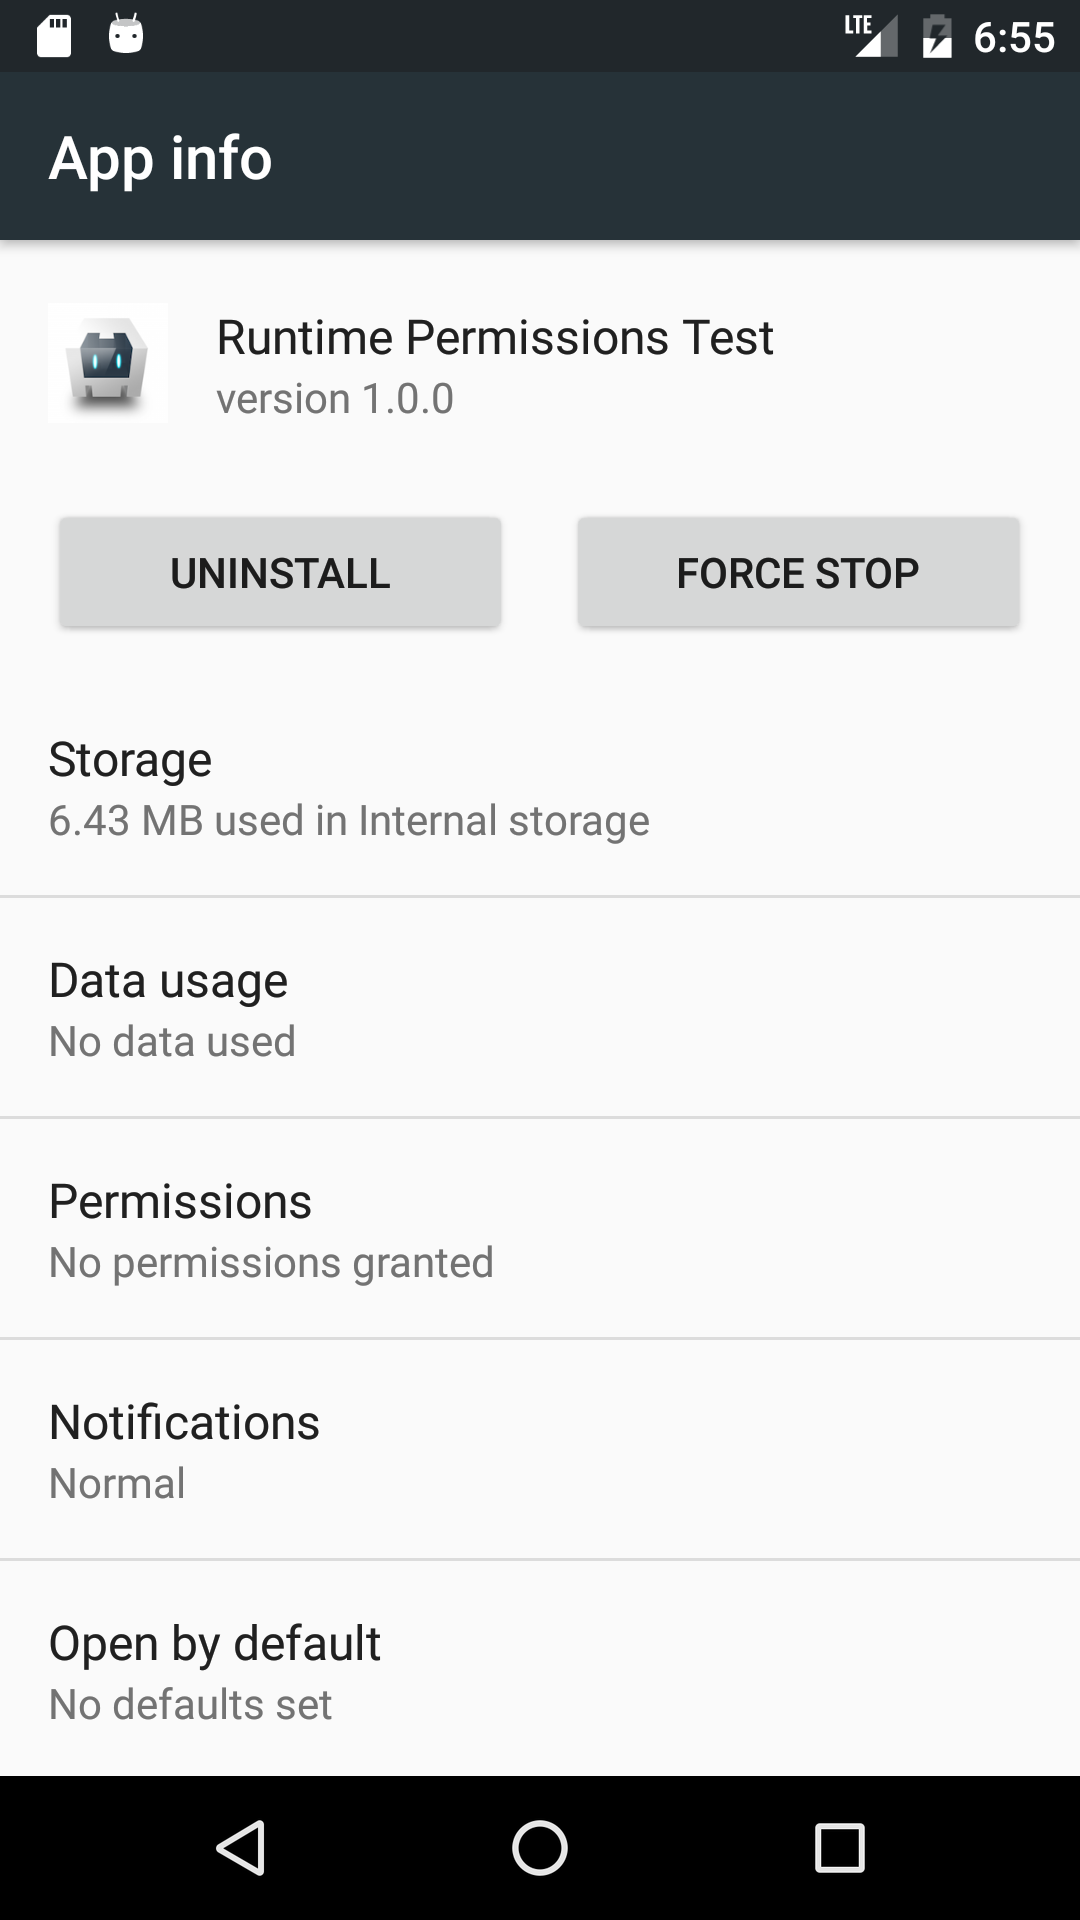
\includegraphics[width=\linewidth]{no_permissions_granted}
		\caption{La aplicación no tiene ningún permiso.}
		\label{fig:ch05:without_permissions}
	\end{subfigure}\pause
	\begin{subfigure}{.23\linewidth}
		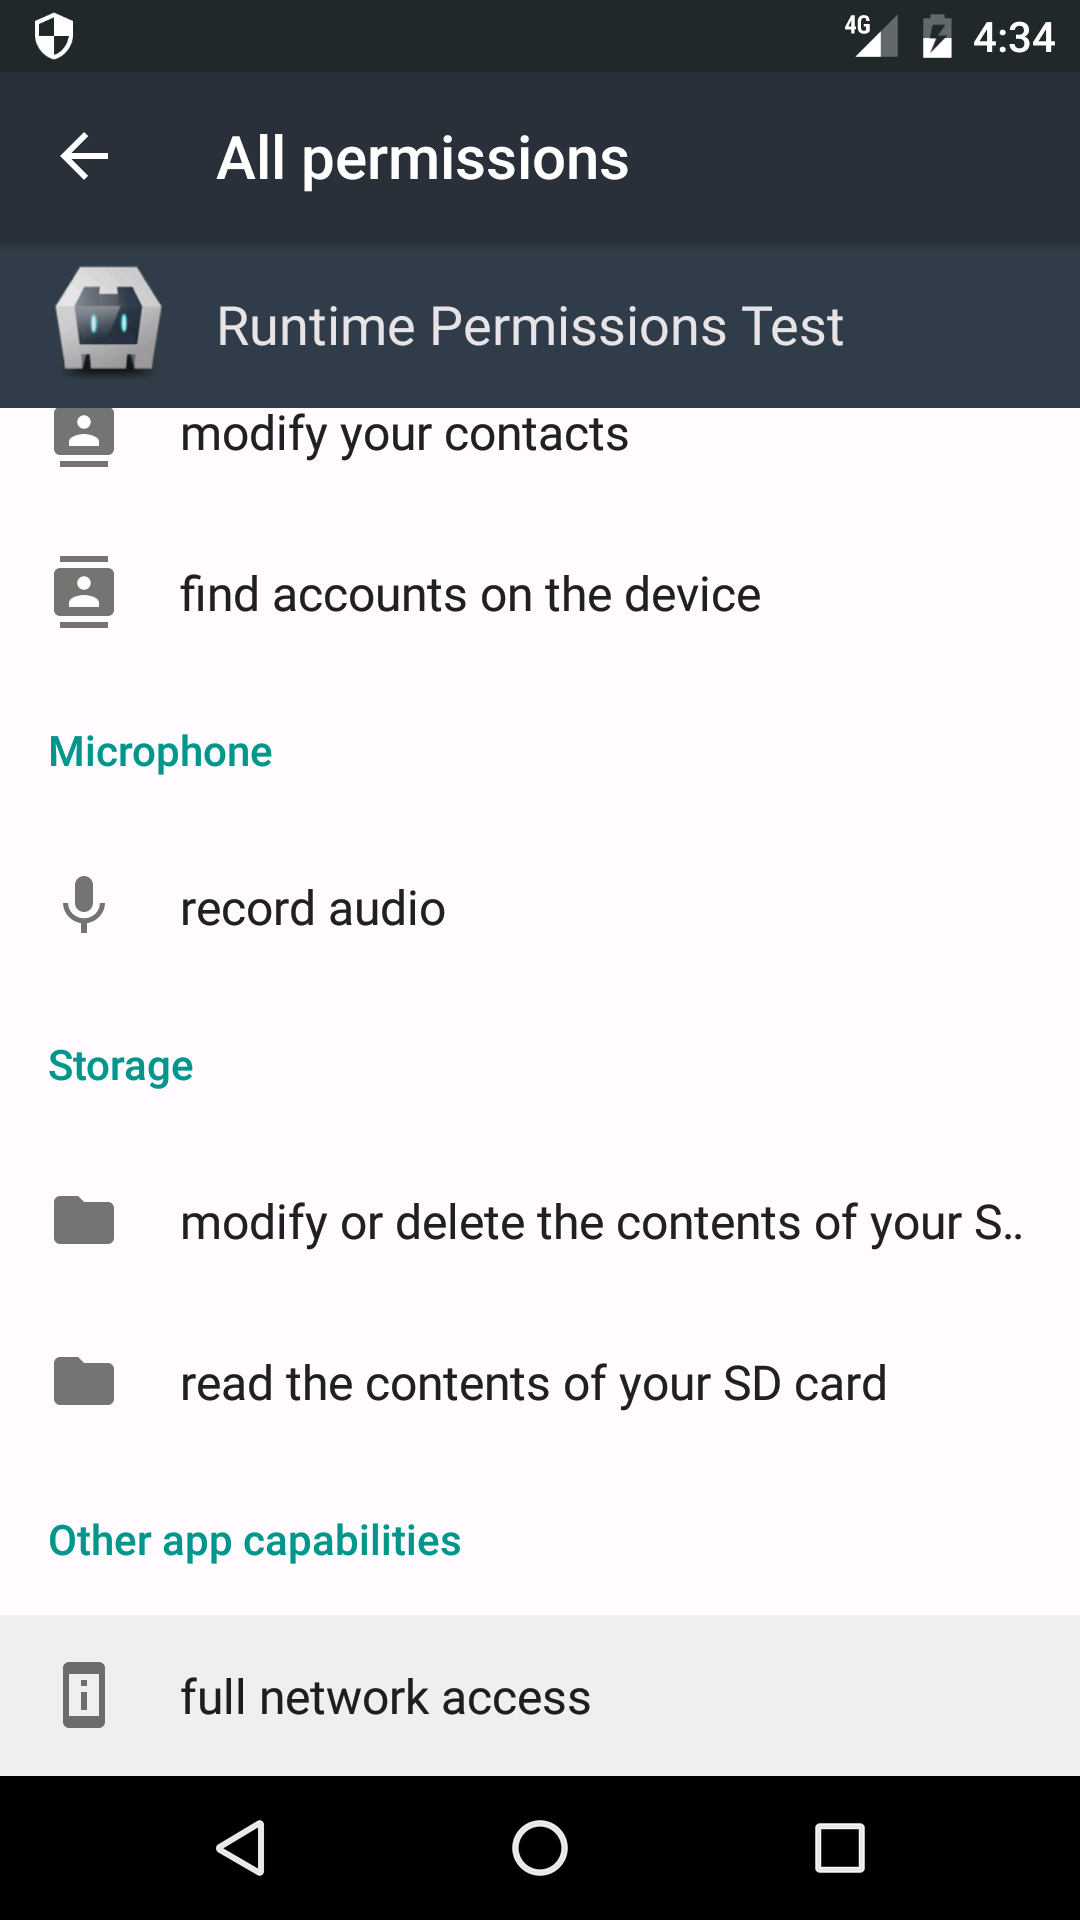
\includegraphics[width=\linewidth]{always_have_internet}
		\caption{Sin embargo, tiene todos los permisos \emph{normales}.}
		\label{fig:ch05:always_have_internet}
	\end{subfigure}
	\caption{Interacción con el usuario en iOS y Android.}
\end{figure}
\end{frame}